%! TEX root = part1.tex
% specify the main TeX file to compile only this subfile
% :h vimtex-tex-root
\documentclass[../main.tex]{subfiles}

\begin{document}


%rmve mycolor when use mybg&bgblock,
%label at first arg.
\begin{frame}[t,mybg=,mycolor=digiPH_leaf,mytitle=center,light]
	\frametitle{Penerapan Bahan Bangunan pada Desain arsitektur}

	\begin{bgblock}{0mm}{0mm}%130x95
		\includegraphics<1>[width=\paperwidth]{81-iHcP}
		\includegraphics<2>[width=\paperwidth]{39-nq6i}
		\includegraphics<3>[width=\paperwidth]{73-Ylnq}
		\includegraphics<4>[width=\paperwidth]{53-GeKm}
		\includegraphics<5>[width=\paperwidth]{17-aApz}
		\includegraphics<6>[width=\paperwidth]{75-wqRU}
	\end{bgblock}
\end{frame}

%rmve mycolor when use mybg&bgblock,
%label at first arg.
\begin{frame}[label=current,t,mybg=,mycolor=digiPH_leaf,mytitle=standard,dark]

	\frametitle{Tanah Soil}
	Lapisan atas dari permukaan bumi, terdiri dari batu hancur dan bahan organik membusuk, yang cocok untuk  pertumbuhan kehidupan tanaman. (Ching, 2012)

	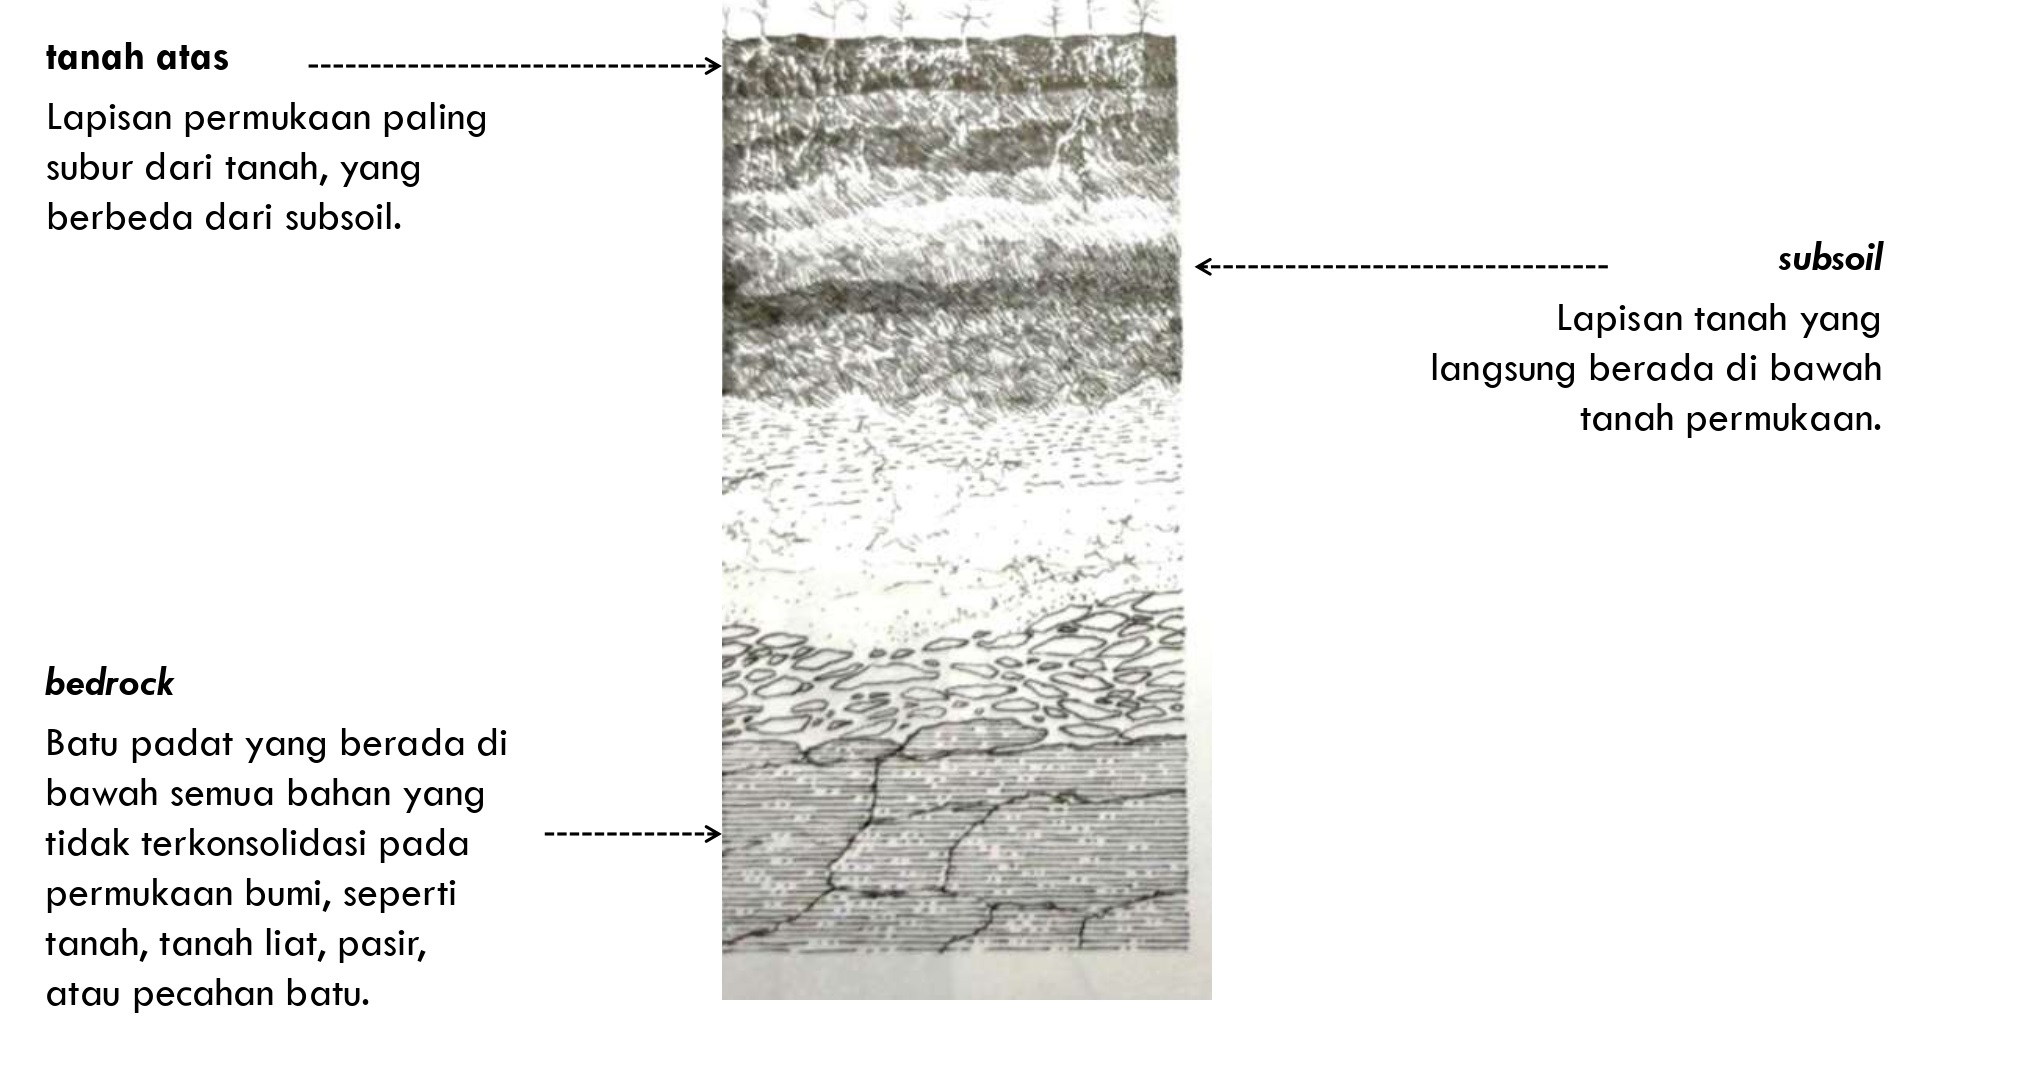
\includegraphics[width=.9\textwidth]{90-WKYX}

\end{frame}

%rmve mycolor when use mybg&bgblock,
%label at first arg.

\begin{frame}[t,mybg=,mycolor=digiPH_ocean,mytitle=standard,dark]
	\frametitle{Kelas tanah}

	Klasifikasi tanah berdasarkan tekstur tanah, digunakan oleh Departemen Agrikultur di AS:  Kerikil, pasir, tanah liat, lempung, lempung dengan sedikit pasir, lanau lempung, tanah liat lempung.
	\includegraphics<1-3>[width=.8\paperwidth]{59-MZ4B}

	\only<1>{
		\begin{columns}
			\begin{column}{0.5\textwidth}
				\small
				\textbf{kerikil}   \\
				Batu-batu kecil, terbentuk secara alami  atau dengan menghancurkan batu.

				\textbf{kerikil hancur}   \\
				Kerikil dengan satu atau lebih  permukaan yang dihasilkan dari  penghancuran mekanis.
			\end{column}
			\begin{column}{0.5\textwidth}
				\small
				\textbf{pea gravel}   \\
				Kerikil alami berdiameter kecil,  biasanya berukuran 6,4 - 9,5 mm.

				\textbf{pebble}   \\
				Batu kecil bulat, terutama yang menjadi  halus karena air.
			\end{column}
		\end{columns}}

	\only<2>{\begin{columns}
			\begin{column}{0.5\textwidth}
				\footnotesize
				\textbf{pasir}   \\Bahan granular lepas yang dihasilkan  dari disintegrasi batu, terdiri dari  butiran yang lebih kecil daripada  kerikil.

				\boldred{lempung pasir}   \\Pasir bernilai baik, terjadi secara alami,  seringkali digunakan sebagai bahan  dasar, memiliki kandungan tanah liat  10\%.

			\end{column}
			\begin{column}{0.5\textwidth}
				\textbf{lanau} \\  Bahan sedimen lepas yang terdiri dari  partikel mineral halus, berdiameter  antara 0,002 mm dan 0,05 mm.
			\end{column}
		\end{columns}}

	\only<3->{\begin{columns}
			\begin{column}{0.5\textwidth}
				\textbf{tanah liat} \\  Bahan tanah alami yang plastis ketika  basah tetapi keras ketika dibakar,  digunakan untuk membuat batu bata,  ubin, atau barang tembikar.

				\boldblue{tanah liat lempung} \\  Tanah dengan 27\% sampai 40\% tanah  liat dan 20\% sampai 45\% pasir.

			\end{column}
			\begin{column}{0.5\textwidth}
				\boldblue{bentonit} \\  Tanah liat yang terbentuk dari  dekomposisi abu vulkanik, memiliki  kemampuan menyerap sejumlah besar  air, dan mengembang beberapa kali  volume naturalnya.

			\end{column}
		\end{columns}}
\end{frame}

\begin{frame}[t,mybg=,mycolor=digiPH_gray,mytitle=imageplus,light]
	\frametitle{Arsitektur tanah liat}
	\begin{bgblock}{0mm}{0mm}%130x95
		\includegraphics<1>[width=\paperwidth]{96-ezSw}
		\includegraphics<2>[width=\paperwidth]{25-ERTb}
	\end{bgblock}

\end{frame}

% \begin{frame}[c,mybg=bg,mycolor=digiPH_gray,mytitle=standard,light]
% 	\frametitle{untitled}
%
% 	\includegraphics[width=40mm]{placeholder}
% \end{frame}

\begin{frame}[t,mybg=,mycolor=digiPH_leaf,mytitle=standard,dark]
	\frametitle{Material tanah liat}
	\begin{columns}
		\begin{column}{0.5\textwidth}
			\boldred{GENTENG TANAH LIAT}

			Kelebihan:
			\begin{itemize}
				\item<1-> Harga yang relatif lebih murah
				\item<1-> Bobotnya cukup ringan
				\item<2-> Daya tekan yang sangat kuat
				\item<2-> Dapat menyerap panas
				\item<3-> Tidak bising saat terkena hujan
				\item<3-> Cenderung lebih awet / tahan lama
			\end{itemize}

			Kekurangan:
			\begin{itemize}
				\item<4-> Rawan bocor bila tidak dirawat
				\item<4-> Mudah berlumut dan berjamur
				\item<5-> Proses pemasangan yang cukup rumit
				\item<5-> Warna yang cepat pudar
			\end{itemize}


		\end{column}
		\begin{column}{0.5\textwidth}
			\rimg{32-1hYi}
		\end{column}
	\end{columns}

\end{frame}

\begin{frame}[label=current,t,mybg=39-nq6i,mytitle=standard,light]
	\frametitle{Batu}
	\utxt{digiPH_navyblue}{digiPH_white}{
		\onslide<1->{Batuan atau sepotong batu yang digali dan dipotong menjadi ukuran dan bentuk tertentu untuk sebuah tujuan  tertentu. (Ching, 2012)}
		\onslide<2->{Batu adalah zat mineral solid yang terbentuk secara alamiah (natural) dan terjadi dalam fragmen atau massa  yang besar. (Ching, 2012)}
	}

	\bimg{.9\textwidth}{56-W38V}

\end{frame}

\begin{frame}[t,mybg=39-nq6i,mytitle=standard,light]
	\frametitle{Batu}

	\includegraphics<1->[width=.9\textwidth]{56-W38V}

	\btxt{digiPH_creamy}{digiPH_black}{
		\begin{columns}

			\begin{column}{0.5\textwidth}
				\only<1-2>{\boldblue{batu sedimen}   \\
					Sebuah kelas batuan yang  terbentuk di permukaan bumi  pada kondisi temperatur dan  tekanan yang rendah.  }
				\only<2->{\boldblue{batuan beku} \\  Sebuah kelas batuan yang  dibentuk dari proses kristalisasi  magma cair, seperti granit.  Biasanya disebut juga sebagai  igneous rock.
				}
			\end{column}


			\begin{column}{0.5\textwidth}
				\only<3->{\boldblue{batu metamorfosis} \\  Sebuah kelas batuan yang telah  melalui proses perubahan dalam  struktur, tekstur, dan komposisi  secara alami, terutama ketika  batuan tersebut menjadi lebih keras  dan berbentuk seperti kristal.}
			\end{column}
		\end{columns}
	}

\end{frame}


\begin{frame}[t,mybg=,mycolor=digiPH_leaf,light]

	\begin{bgblock}{0mm}{0mm}%130x95
		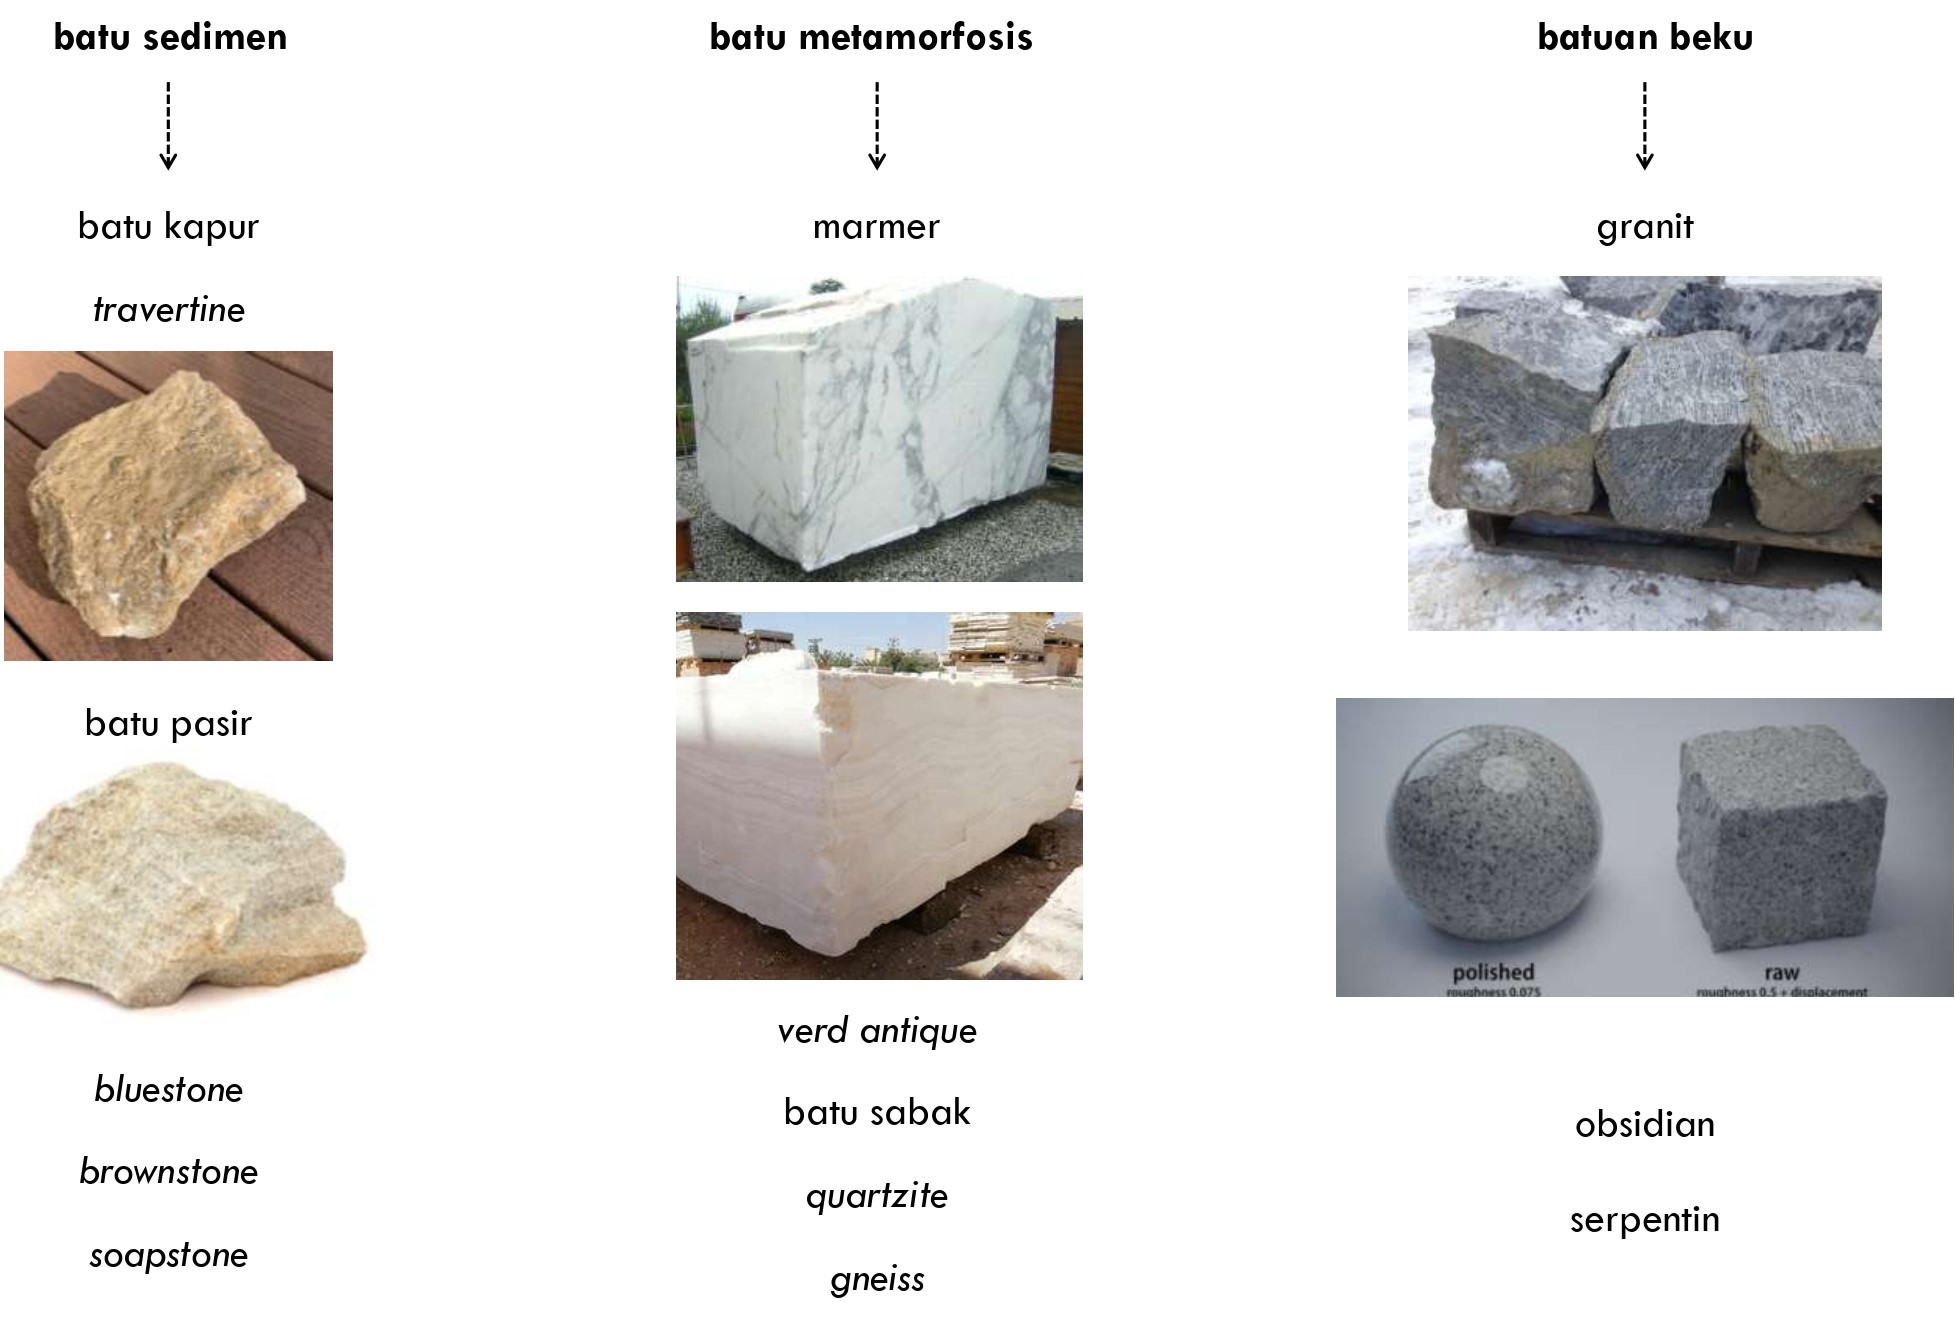
\includegraphics[width=\paperwidth]{87-MHOZ}
	\end{bgblock}
\end{frame}

\begin{frame}[t,mybg=,mycolor=digiPH_ocean,mytitle=standard,dark]
	\frametitle{Arsitetur Batu}

	\begin{bgblock}{0mm}{0mm}%130x95
		\includegraphics<1>[width=\paperwidth]{89-Hyct}
		\includegraphics<2>[width=\paperwidth]{93-kU53}
		\includegraphics<3>[width=\paperwidth]{27-Gl6g}

	\end{bgblock}
\end{frame}

\begin{frame}[t,mycolor=digiPH_leaf,mytitle=standard,dark]
	\frametitle{Sifat-sifatBatu}

	\only<1->{\utxt{digiPH_gray}{digiPH_black}{Sifat batu dibedakan menjadi dua, yaitu sifat fisik dan sifat mekanik. Sifat fisik adalah  sifat yang tampak pada batu. Sedangkan sifat mekanik adalah kekuatan batu dalam  menahan gaya.}}

	\btxt{digiPH_gray}{digiPH_black}{\boldblue{SIFAT FISIK BATU:} \\
		\only<2>{
			\begin{itemize}
				\item Massa jenis atau kerapatan (density) atau berat batuan tersebut tiap  satuan volume;
				\item Porositas atau perbandingan volume pori-pori batuan dengan volume total  batuan;
				\item Kekerasan (hardness)
			\end{itemize}}

		\only<3>{
			\begin{itemize}
				\item Abrasivitas atau tingkat pengikisan yang dapat dialami oleh batu ketika  bersentuhan dengan material lain;
				\item Permeabilitas atau kemampuan batuan menghantarkan fluida;
				\item Kecepatan gelombang pada batu (menunjukkan susunan butir-butir  penyusun batuan, semakin cepat, maka susunannya semakin rapat).
			\end{itemize}
		}
	}

\end{frame}


\begin{frame}[label=current,t,mybg=bg,mycolor=digiPH_gray,mytitle=standard,light]
	\frametitle{Sifat-sifat Batu}

	\only<1->{\utxt{digiPH_gray}{digiPH_black}{Sifat batu dibedakan menjadi dua, yaitu sifat fisik dan sifat mekanik. Sifat fisik adalah  sifat yang tampak pada batu. Sedangkan sifat mekanik adalah kekuatan batu dalam  menahan gaya.}}

	\btxt{digiPH_gray}{digiPH_black}{\boldblue{SIFAT MEKANIK  BATU:} \\
		\only<2>{\begin{itemize}
				\item Kekuatan tekan (compressive strength)    menyatakan sifat ketahanan suatu batuan terhadap tekanan / kompresi yang    berada pada satu garis lurus
				\item Kekuatan tarik (tensile strength)     menyatakan sifat kekuatan benda terhadap gaya tarik
			\end{itemize}}


		\only<3>{\begin{itemize}
				\item Modulus elastisitas    adalah perbandingan antara regangan dan tegangan dari suatu benda, selama    gaya yang bekerja tidak melampaui batas elastisitasnya
				\item Regangan maksimum (strain at failure)    menunjukkan besarnya perubahan panjang maksimum yang dapat dialami oleh s uatu    benda yang mengalami gaya tarik
			\end{itemize}}

		\only<4>{\begin{itemize}
				\item Point load strength index     menyatakan gaya yang dapat disokong oleh suatu batuan dengan menggunakan    perbandingan antara gaya maksimum yang mampu diterima dengan luas  permukaan    dari batuan tersebut
				\item Ketangguhan batu (fracture toughness)    menunjukkan kemampuan batu menahan gaya sebelum terjadi patahan atau    retakan
			\end{itemize}}
	}

\end{frame}




\begin{frame}[t,mybg=bg,mycolor=digiPH_leaf,mytitle=standard,dark]
	\frametitle{Buku referensi}
	\begin{itemize}
		\item Winoto, Agnes D.Y., 2014, Ilmu Bahan Bangunan, TAKA publisher.
		\item Ching, Francis DK., 2014, Kamus Visual Arsitektur Edisi 02, Penerbit Erlangga
	\end{itemize}
\end{frame}














\end{document}
